\section{Preliminaries}







\subsection{Problem Setup}


We consider the following least squares approximation problem:

\begin{equation}\label{eq:leastsquares}
\begin{aligned}
    &\min_{\bm \theta} L(\bm \theta) =  \frac{1}{2} \sum_{j=1}^s |f_{\bm \theta}(x_j) - y_j|^2,\\
    &\mbox{ where } \,\,\, f_{\bm \theta}(x) = \sum_{i=1}^m c_i [a_i x + b_i]_+, \quad \bm \theta = (\bm a \in \RR^m, \bm b \in \RR^m, \bm c \in \RR^m),
\end{aligned}
\end{equation}

where $S = \{ (x_i, y_i) \in \RR^2, \, i =1,\ldots, s\}$ is a given set of samples. Our functional space $\mathcal F_m = \{f_{\bm \theta}: \RR\rightarrow \RR, \, \,\textbf{} {\bm \theta} \in \RR^{3m}\}$ is the family of 1D feedforward shallow ReLU networks with exactly $m$ neurons. It is easy to see that $\mathcal F_m$ is contained in the the set $CPL_m$ of \emph{continuous piecewise-linear} functions with at most $m$ knots. The knots of $f_{\bm \theta}$ are the points where the operand inside a ReLU activation changes sign:

\begin{equation}\label{eq:knots}
e_i = -\frac{b_i}{a_i}, \quad a_i \ne 0, \quad i=1,\ldots,m.
\end{equation}

See Figure~\ref{fig:knots} for an example of a function $f_{\bm \theta}$ and its knots. In this paper, we focus on the overparameterized setting $m \gg s$. Although $\mathcal F_m$ is a strict subset of $CPL_m$, it contains $CPL_{m-1}$ (see Appendix ...). In particular, many parameter values can interpolate the samples and have zero loss $L(\bm \theta) = 0$.

\begin{figure}
    \centering
    \minipage{0.5\textwidth}
    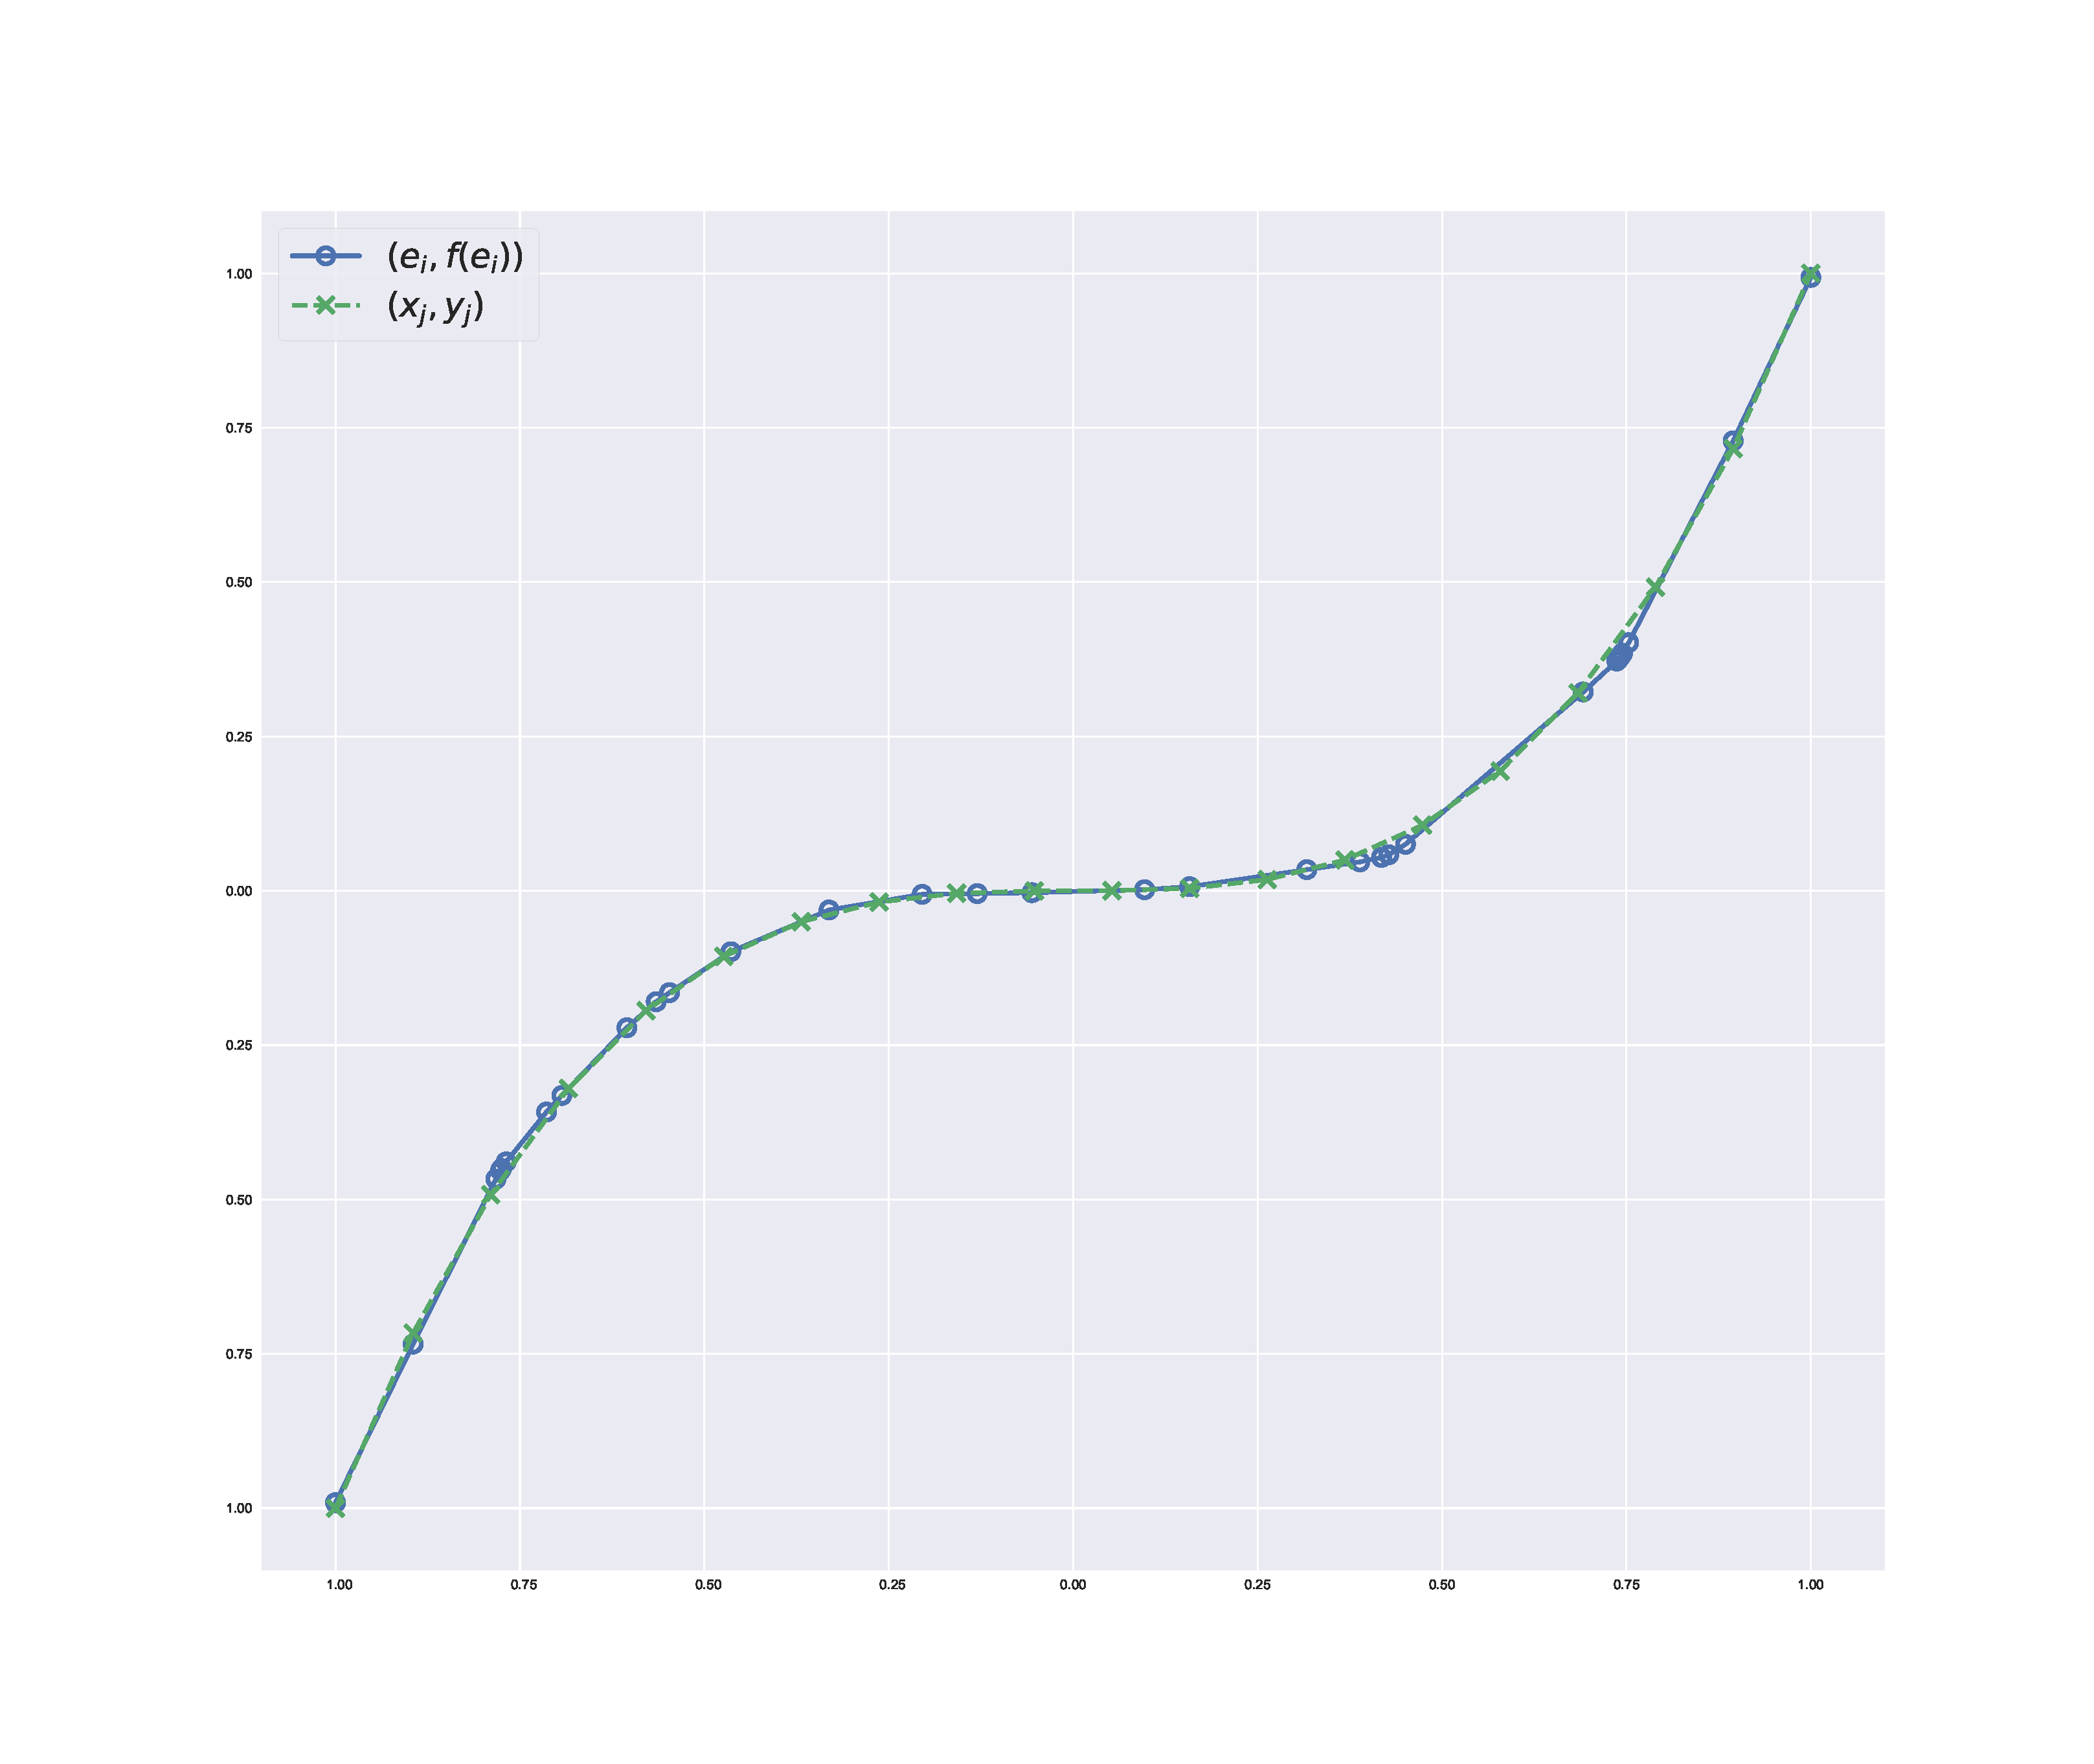
\includegraphics[width=\textwidth]{figures/knots2.pdf}
    \endminipage\hfill
    \minipage{0.5\textwidth}
    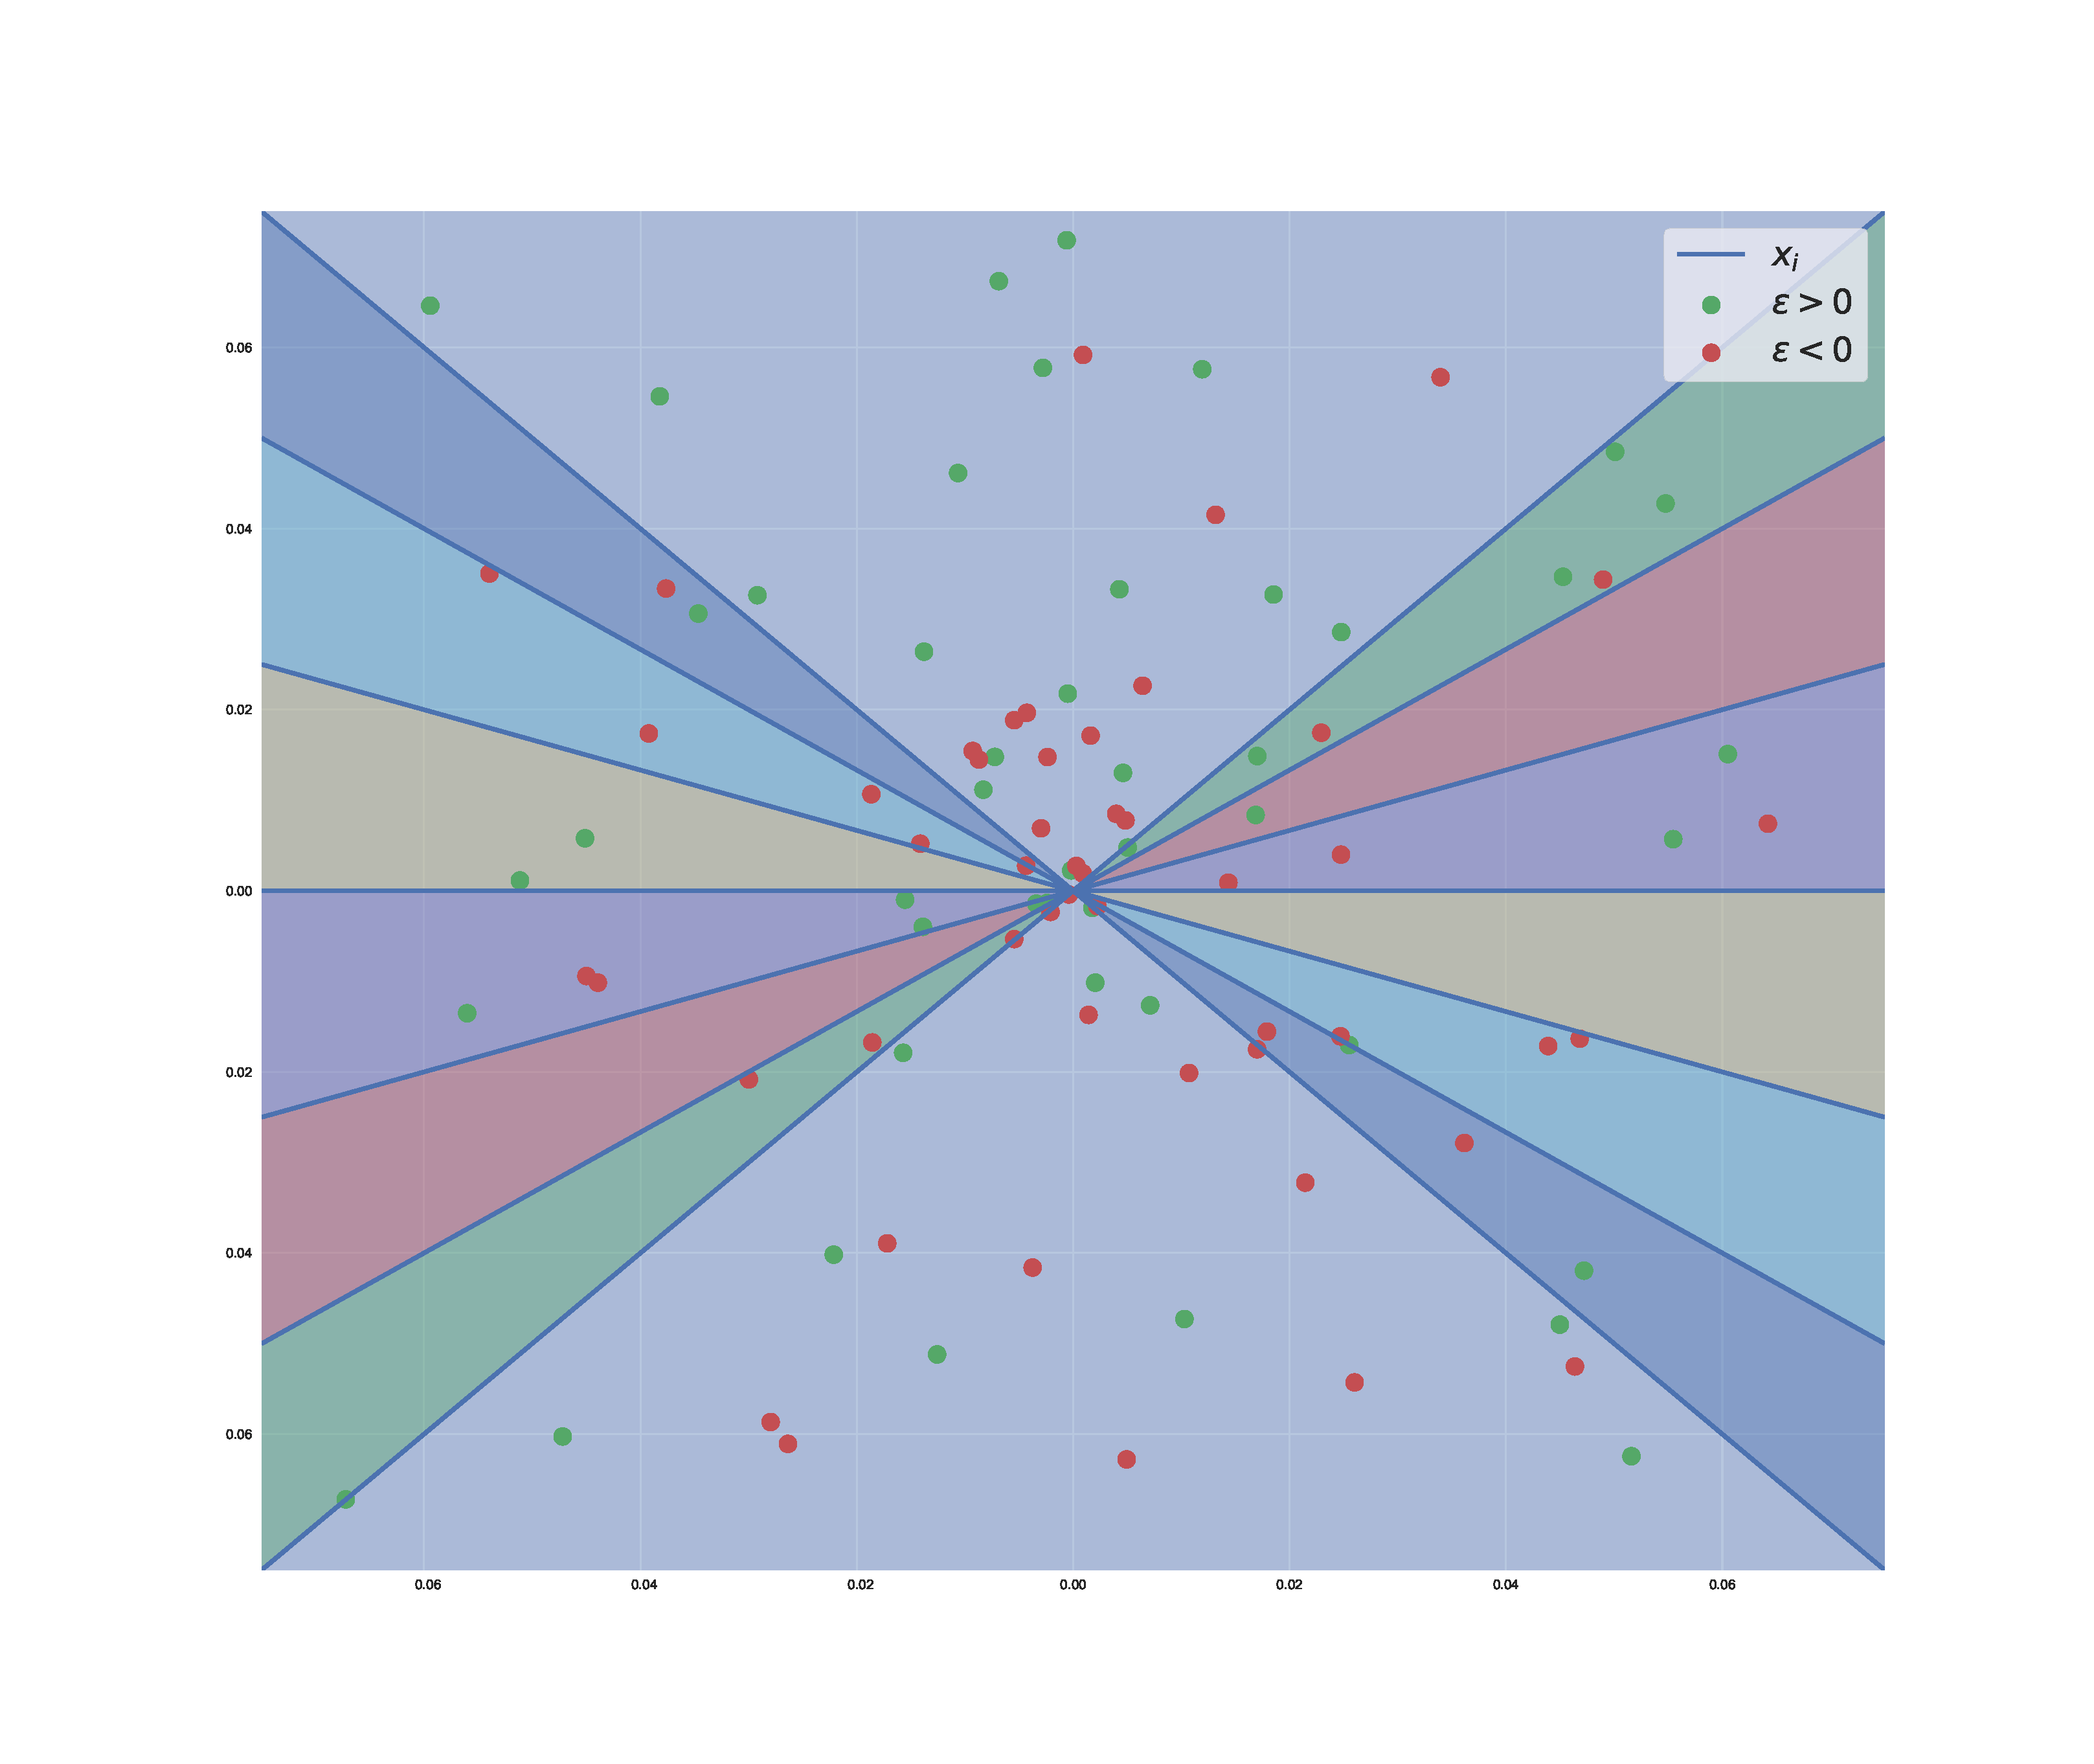
\includegraphics[width=\textwidth]{figures/phaseplot_eg.pdf}
    \endminipage\hfill
    
    
    \caption{The input samples $(x, y) = (x_j, y_j)_{j=1}^s$ (blue x's) to which we fit a neural network, $f(x)$ \eqref{eq:ReLU1D} using the least squares loss \eqref{eq:leastsquares}. The function $f(x)$ is piecewise linear with the boundaries between pieces occurring at $(e_i, f(e_i)) = (\frac{-b_i}{a_i}, f(\frac{-b_i}{a_i}))_{i=1}^m$ (green circles). These points correspond to when the operand to one of the ReLUs in \eqref{eq:ReLU1D} becomes active or inactive.}
    \label{fig:knots}
\end{figure}
% \begin{figure}
%     \centering
%     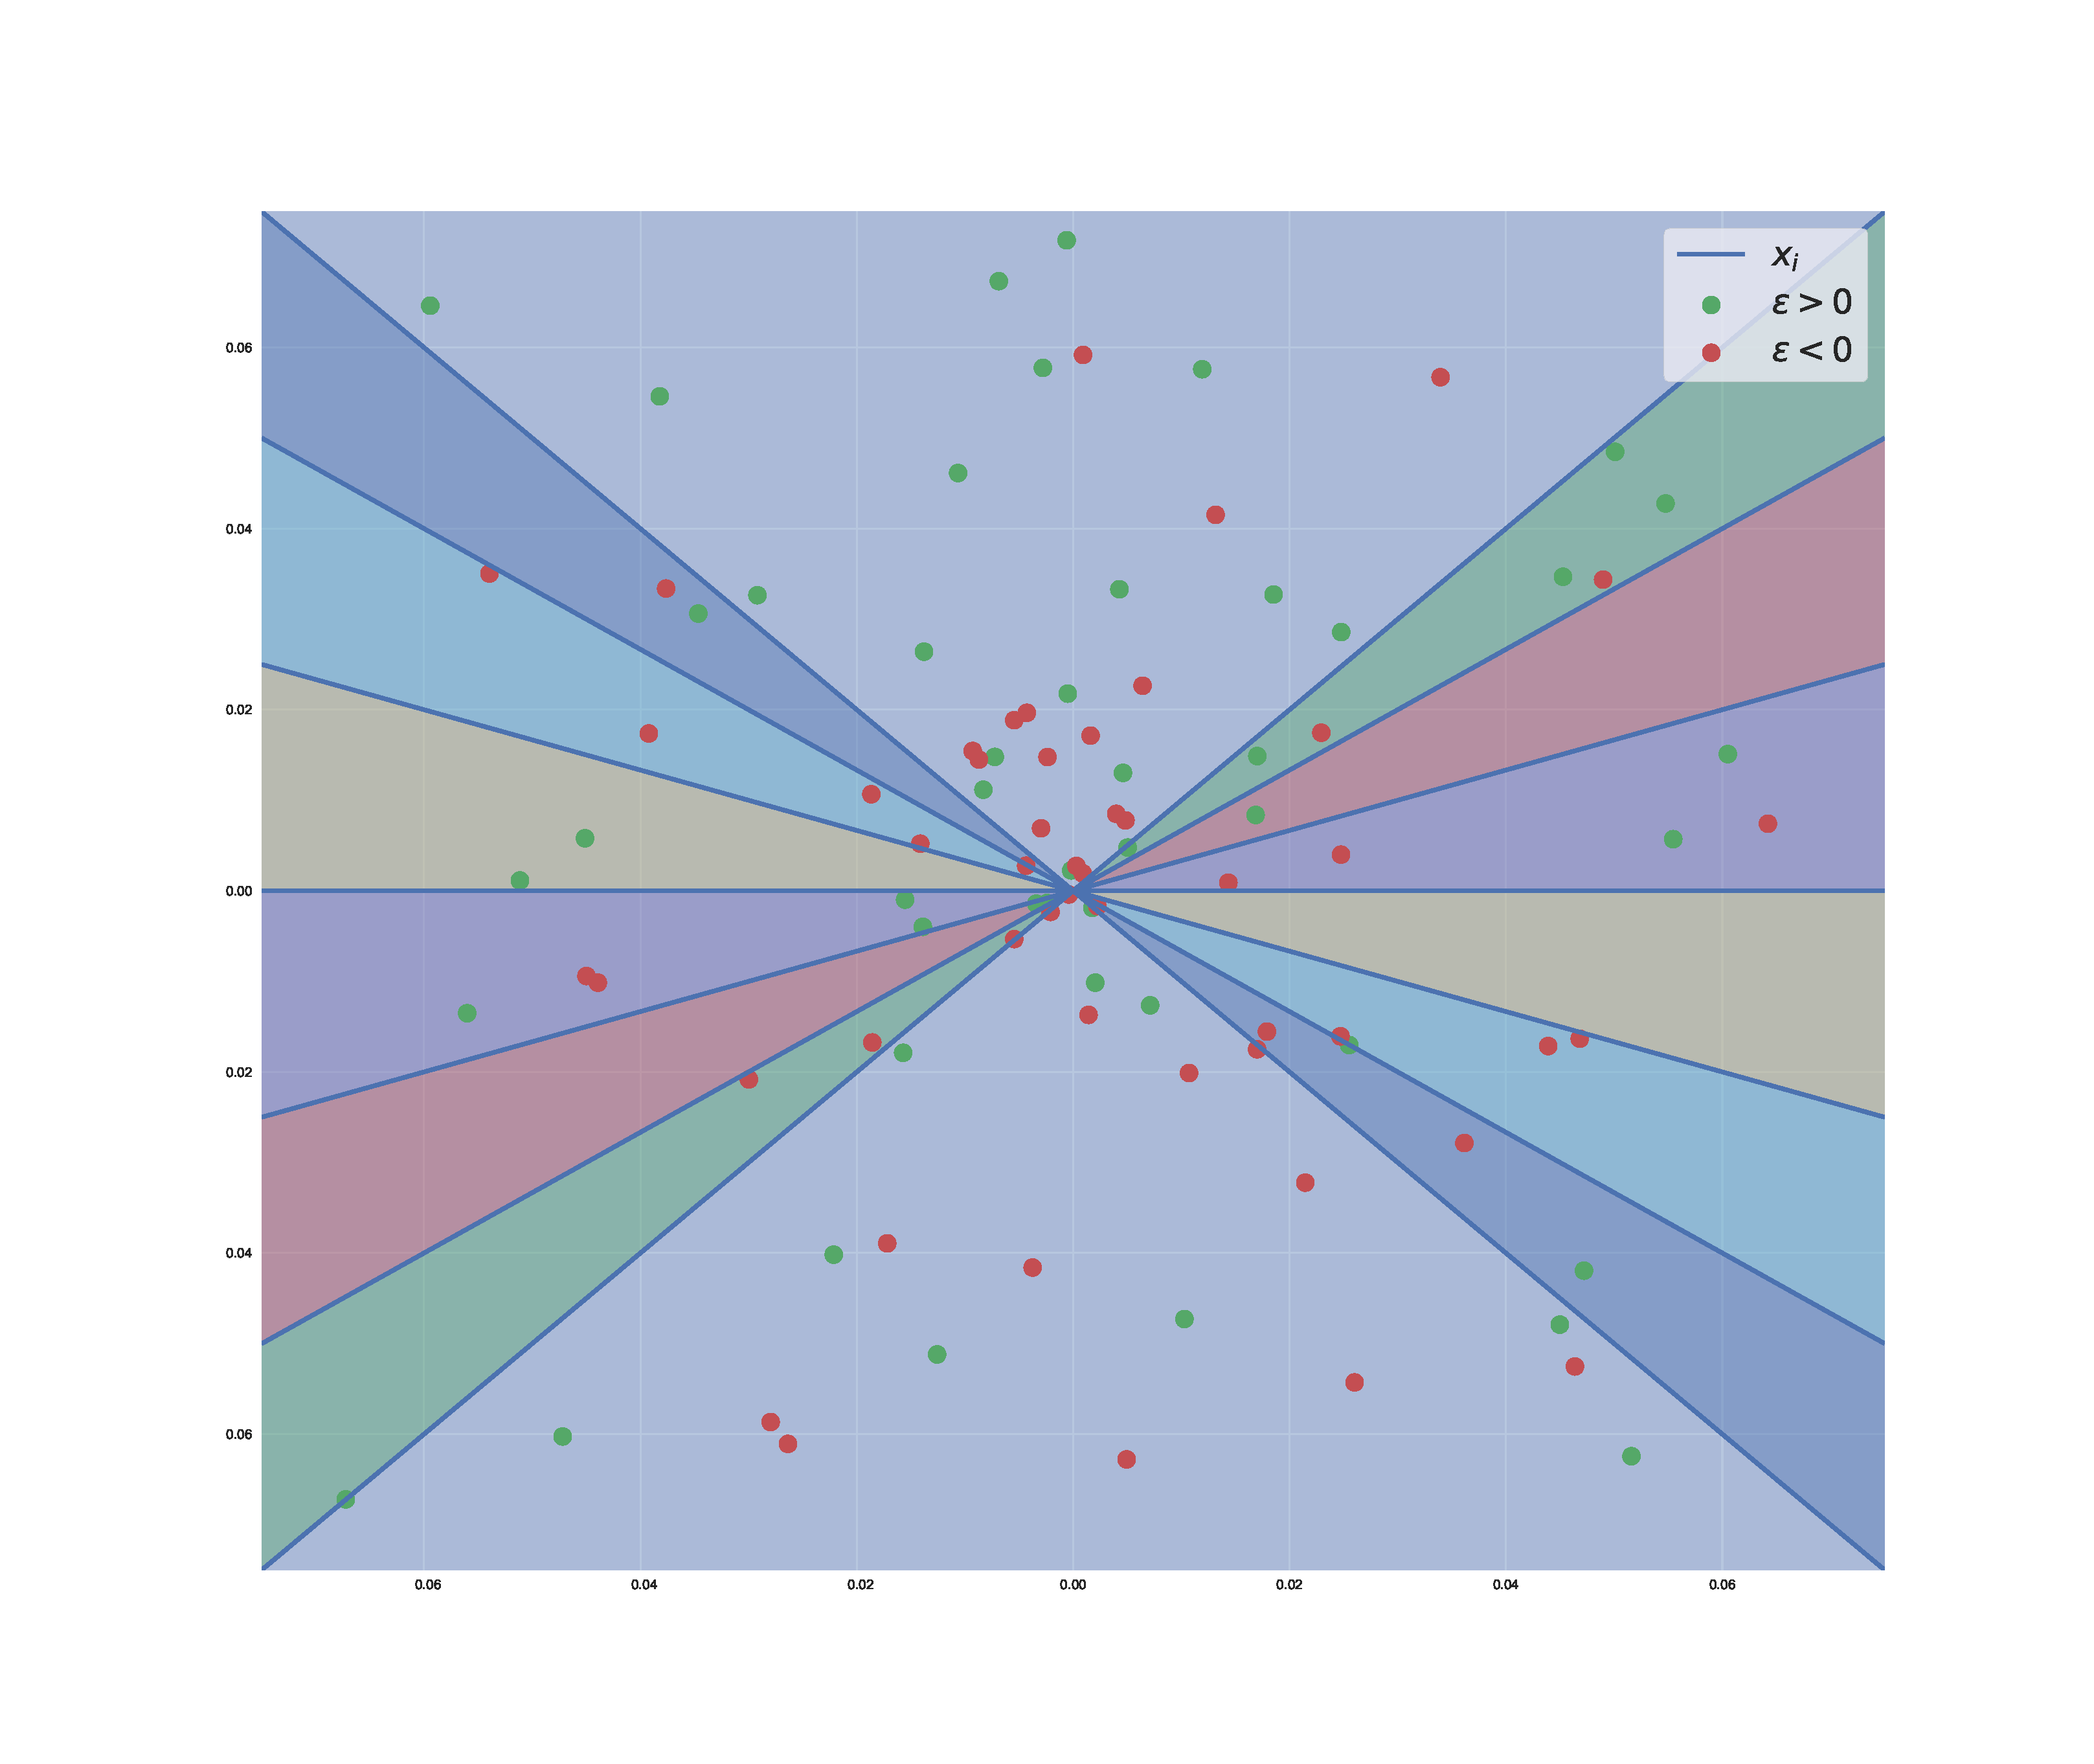
\includegraphics[width=.5\textwidth]{figures/phaseplot_eg.pdf}
%     \caption{Example plot of neurons in \emph{reduced parameter space}. The green dots are the neurons $(u_i, v_i)$ for which $c_i$ is positive and the red knots are those for which $c_i$ is negative. The knot for a neuron $(u_i, v_i)$ lies on a sample $x$ if it intersects the line $-\frac{v_i}{u_i} = e_i = x$. The blue lines correspond to the sample positions. Note that the activation of a neuron will change when it crosses a sample boundary.}
%     \label{fig:phaseplot_eg}
% \end{figure}


\subsection{Gradient flow}

Our goal is to solve \eqref{eq:nnloss} using the \emph{gradient flow} (the continuous-time limit of gradient descent) of the least squares loss:

\begin{equation}\label{eq:gradient_flow}
    \bm \theta(0) = \bm \theta_0, \qquad \bm \theta'(t) \in \partial L(\bm \theta(t)).
\end{equation}

Here $\partial L(\bm \theta)$
% $\partial L(\bm \theta) = \{\bm p \in \RR^{3m} , L(\bm \theta') \ge L(\bm \theta) + \bm p \cdot (\bm \theta' - \bm \theta) \qquad \forall \bm \theta' \}$ 
denotes the \emph{Clarke subdifferential}~\cite{clarke1975generalized}, since $L(\bm \theta)$ is only piecewise smooth. At generic smooth points $\bm \theta$, the subdifferential coincides with the gradient $\partial L(\bm \theta(t)) = \{\nabla L(\bm \theta)\}$. However, we argue in \todo{Section ...} that the discontinuities of the gradient play an important role in the dynamics in practice. For this reason, we subdivide the parameter space into \emph{regions} associated with different \emph{activation patterns}:\note{we should probably allow $c=0$ and then properly define the interior of a region} \todo{Reference the figure here}

\begin{equation}
    R(\bm \tau,\bm \epsilon) = \{\bm \theta = (\bm a, \bm b, \bm c) \in \RR^{3m} \, | \, \mathds 1 [a_j x_i + b_j \ge 0] = \tau_{ij},\, {\rm sign}(c_j) = \epsilon_j\}, \quad \bm \tau \in \{0,1\}^{s \times m}, \bm \epsilon \in \{-1,1\}^{m}.
\end{equation}

If $R(\bm \tau, \bm \epsilon)$ is not empty, it is a polyhedral cone containing the origin, and it is a product of ``sectors'' corresponding to the activation pattern of each neuron. It is important to note that, in our one-dimensional setting, every neuron can have \emph{at most} $2s$ activation patterns (out of the possible $2^s$ combinatorial types), which means that, for $R(\bm \tau, \bm \epsilon)$ to be non-empty, the columns of $\bm \tau$ must be chosen among $2s$ possible vectors.
In the interior of a non-empty region $R(\bm \tau, \bm \epsilon)$, the gradient of $L(\bm \theta)$ can be written as
\begin{equation}\label{eq:derivative_equations}
\begin{aligned}
&\nabla_{a_i}L(\bm \theta) = c_i \sum_{j=1}^s \tau_{ij} x_j r_j,\\
&\nabla_{b_i}L(\bm \theta) = c_i \sum_{j=1}^s \tau_{ij} r_j,\\
&\nabla_{c_i}L(\bm \theta) = \sum_{j=1}^s \tau_{ij} (a_i x_j + b_i) r_j,\\
\end{aligned}
\end{equation}
where $r_j = f_{\bm \theta}(x_j) - y_j$ is the $j$-th \emph{residual}. Finally, we remark that a solution $\bm \theta(t)$ to~\eqref{eq:gradient_flow} will in general converge to a first-order stationary point $\bm \theta^*$ where $0 \in \partial L(\bm \theta^*)$. For certain asymptotic (highly over-parameterized) regimes, it is possible to show convergence to global optima~\cite{du2018gradient,chizat2018global}. In our concrete low dimensional setting, we can state the following result.

\begin{proposition} Let $\bm \theta^* = (\bm a^*, \bm b^*, \bm c^*)$ be a critical point for $L(\bm \theta)$, and consider the matrix
\begin{equation}
    \bm M_{\bm a^* \bm b^*} = \big [ [a_j^* x_i + b_j^*]_+ \big ]_{ij} \in \RR^{s \times m}.
\end{equation}
If $\bm M_{\bm a^* \bm b^*}$ has full rank, then $L(\bm \theta^*) = 0$, so $\bm \theta^*$ is a global minimum. If $s< m$ and $e_1 \le \ldots \le e_m$ are the knots~\eqref{eq:knots} associated with $\bm \theta^*$, then a sufficient condition for $\bm M_{\bm a^* \bm b^*}$ to have full rank is that each interval $[-\infty, e_1],[e_1,e_2],\ldots,[e_m,\infty]$ contains at most one sample point $x_i$.
\end{proposition}





\subsection{Visualization of reduced parameters}


In the next section, we will illustrate our results by visualizing neurons as in Figure~\ref{fig:phaseplot_eg}. Here, every colored ``particle'' represents a single neuron of $f_{\bm \theta}$ using \emph{reduced coordinates} $\bm \xi$:
\begin{equation}\label{eq:reduced_params}
\bm \xi_i = (u_i,v_i) = (|c_i|a_i,|c_i| b_i), \qquad i=1,\ldots,m.
\end{equation}
The color of the particle indicates the sign $\epsilon_i \in \{+1,-1\}$ of $c_i$ (assuming it is non-zero). Each data point $x_i$ corresponds to a \emph{line} through the origin, namely $u x_i + v =0$. The $2s$ colored sectors indicate regions where neurons have a fixed activation patterns.

Note that although the reduced coordinates $(u_i,v_i)$ do not uniquely identify the parameters $(a_i,b_i,c_i)$, together with $\epsilon_i$ they determine the neuron as a \emph{function}, since $c_i[a_i x + b_i]_+ = \epsilon_i[u_i x + v_i]_+$.
Thus, the reduced parameters determine $f_{\bm \theta}$, but have $m$ fewer degrees of freedom (one per neuron) compared to $\bm \theta$. These degrees of freedom are indeed unnecessary because the association $\bm \theta \rightarrow f_{\bm \theta}$ is not injective. 

% On the other hand, we will argue in the next section that the knowledge of the initial parameters $\bm \theta(0)$ is sufficient recover  to ``lift'' a reduced representation and recover the true neurons.


